\documentclass[10pt,letterpaper,twoside]{article}
\usepackage{code/manuscript_assets/researchpreprint}
\usepackage{amsmath,amssymb,amsthm,booktabs,caption,float,graphicx,microtype}
\usepackage[hidelinks]{hyperref}
\captionsetup{font=small,labelfont=bf,width=0.92\textwidth}

\newcommand{\PersistenceRows}{%
development decoder & 1 & 13--15 & 6.63e-05 & stationary toggle fit & 1.15e-04 & 42.3\% \\
development decoder & 2 & 15--17 & 5.26e-05 & stationary toggle fit & 1.35e-04 & 61.2\% \\
development decoder & 3 & 17--19 & 5.66e-05 & stationary toggle fit & 1.39e-04 & 59.4\% \\
development decoder & 4 & 19--25 & 9.00e-05 & stationary toggle fit & 1.40e-04 & 35.8\% \\
confirmation decoder & 1 & 13--15 & 5.80e-05 & stationary toggle fit & 1.10e-04 & 47.4\% \\
confirmation decoder & 2 & 15--17 & 5.54e-05 & stationary toggle fit & 1.33e-04 & 58.4\% \\
confirmation decoder & 3 & 17--19 & 6.95e-05 & stationary toggle fit & 1.30e-04 & 46.4\% \\
confirmation decoder & 4 & 19--25 & 8.94e-05 & stationary toggle fit & 1.03e-04 & 13.0\% \\
}
\newcommand{\PersistenceHash}{fb0ff77517c4acb9f59104dbc10cb125e5b992f4e45076afdc7cf7aae070cc6c}


\newtheorem{theorem}{Theorem}
\newtheorem{proposition}{Proposition}
\newcommand{\R}{\mathbb{R}}
\newcommand{\norm}[1]{\left\lVert#1\right\rVert}

\hypersetup{
 pdftitle={Effective-Toggle Persistence for Rolling Forecasts of Surface-Code Logical Error Rates},
 pdfauthor={Molena Huynh}
}

\begin{document}

\title{Effective-Toggle Persistence for Rolling Forecasts\\
of Surface-Code Logical Error Rates}
\author{Molena Huynh}
\email{molena.huynh@jmp.com}
\affiliation{North Carolina State University}
\date{}
\maketitle

\begin{abstract}
Logical error rates accumulated over repeated error-correction rounds are
bounded probabilities with a known parity geometry. A stationary per-round
toggle model respects that geometry but fails on the public Google surface-code
hardware record: the effective toggle inferred from measured rates changes
systematically with circuit depth. This paper introduces effective-toggle
persistence, a rolling forecast that inverts the most recent rate within each
hardware stratum and propagates that effective toggle analytically to later
rounds. The method requires no numerical optimization. The analysis proves
exactness under stationary toggles, an $r$-Lipschitz error bound under drift,
and $O(N+G)$ work with $O(G)$ storage for $N$ records and $G$ strata. The
protocol uses 130 hardware experiments, 50,000 shots per experiment, two code
distances, two logical bases, and thirteen round settings. Tensor-network
decoder rates define development; belief-matching decoder rates are reserved
as a distinct confirmation endpoint. Across four rolling folds, the proposed
forecast reduces mean-squared error relative to the strongest of a stationary
toggle fit, nearest-round rate, and ridge extrapolation by 35.8--61.2 percent
on development and 13.0--58.4 percent on confirmation. It wins every fold.
The measured implementation is over three orders of magnitude faster than the
registered grid fit at ten strata, while the nearest-rate baseline remains
faster and substantially less accurate. The result is a hardware-record
forecasting statement, not a stationary noise-model validation.
\end{abstract}

\noindent\textbf{Keywords.} surface code; logical error rate; rolling forecast;
parity model; calibration; reproducible hardware data.

\section{Introduction}

Repeated rounds of quantum error correction convert local faults into a
depth-dependent logical failure probability. Decoder comparisons and scaling
studies therefore require forecasts that respect both probability bounds and
the accumulation geometry. The independent-toggle curve
\begin{equation}
 h_r(q)=\frac{1-(1-2q)^r}{2},\qquad q\in[0,1/2],
 \label{eq:toggle}
\end{equation}
is a natural baseline: $q$ is a per-round toggle probability and $h_r(q)$ is
the probability of odd parity after $r$ rounds. A single $q$ for all depths in
a hardware stratum is, however, a stationarity assumption rather than a
consequence of the code.

The public Google surface-code record~\cite{google2023suppressing} contains
logical error rates across circuit depths, logical bases, code distances, and
patch locations. Direct inversion of \eqref{eq:toggle} reveals a pronounced
depth dependence in the effective per-round toggle. A stationary curve
consequently underpredicts later-round error. Linear extrapolation ignores the
bounded parity geometry, while carrying forward the last observed logical rate
ignores continued accumulation.

Effective-toggle persistence combines the strongest element of both baselines.
Within each declared hardware stratum it takes the most recent observed rate,
maps that rate to its exact effective toggle, and evaluates
\eqref{eq:toggle} at future depths. The estimator has one state value per
stratum, no fitted trend, no grid search, and no dense matrix. Its error is
controlled directly by drift of the effective toggle.

The evaluation separates decoder endpoints. Tensor-network decoder rates are
used to formulate and assess the method. Belief-matching decoder rates are
then processed with the unchanged estimator, strata, folds, and baselines.
Every fold trains only on earlier circuit depths.

\section{Parity geometry and persistence}

\subsection{Toggle identity}

\begin{theorem}[Odd-parity probability]
\label{thm:parity}
Let $X_1,\ldots,X_r$ be independent Bernoulli variables with
$\Pr(X_i=1)=q$. Then
\begin{equation}
 \Pr\!\left(\sum_{i=1}^r X_i\equiv1\pmod 2\right)=h_r(q).
 \label{eq:odd}
\end{equation}
\end{theorem}

\begin{proof}
Since $(-1)^{\sum_iX_i}$ equals $1$ for even parity and $-1$ for odd parity,
\begin{align}
 \mathbb E\!\left[(-1)^{\sum_iX_i}\right]
 &=\prod_{i=1}^r\mathbb E[(-1)^{X_i}]
 =(1-2q)^r.
\end{align}
Writing $P_{\rm even}+P_{\rm odd}=1$ and
$P_{\rm even}-P_{\rm odd}=(1-2q)^r$ gives
$P_{\rm odd}=[1-(1-2q)^r]/2$.
\end{proof}

For $p\in[0,1/2]$, \eqref{eq:toggle} is strictly increasing and has inverse
\begin{equation}
 h_r^{-1}(p)=\frac{1-(1-2p)^{1/r}}{2}.
 \label{eq:inverse}
\end{equation}
The value $q_r=h_r^{-1}(p_r)$ is termed the effective toggle at depth $r$.
It is an exact reparameterization of the measured rate; it is not assumed to be
constant.

\subsection{Rolling estimator}

Let $g\in\{1,\ldots,G\}$ index strata defined by logical basis, code distance,
and patch center. At forecast origin $r_0$, let $p_{g,r_0}$ be the mean of all
records in stratum $g$ at the latest available round. Define
\begin{equation}
 \widehat q_g=h_{r_0}^{-1}(p_{g,r_0}),
 \qquad
 \widehat p_{g,r}=h_r(\widehat q_g),\quad r>r_0.
 \label{eq:persistence}
\end{equation}
Ties at $r_0$ are averaged before inversion. This makes the estimator
invariant to row ordering.

\begin{theorem}[Exactness and drift bound]
\label{thm:drift}
Suppose the true rate in one stratum has representation
$p_r=h_r(q_r)$. The forecast \eqref{eq:persistence} satisfies:
\begin{enumerate}
\item If $q_r=q_{r_0}$, then $\widehat p_r=p_r$.
\item For arbitrary $q_r,q_{r_0}\in[0,1/2]$,
\begin{equation}
 |\widehat p_r-p_r|\le r|q_{r_0}-q_r|.
 \label{eq:drift-bound}
\end{equation}
\end{enumerate}
\end{theorem}

\begin{proof}
The first statement follows from
$h_{r_0}^{-1}(h_{r_0}(q_{r_0}))=q_{r_0}$ and evaluation at $r$. For the
second, differentiation of \eqref{eq:toggle} gives
\begin{equation}
 h_r'(q)=r(1-2q)^{r-1}.
\end{equation}
Hence $0\le h_r'(q)\le r$ on $[0,1/2]$. The mean-value theorem yields
\begin{equation}
 |h_r(q_{r_0})-h_r(q_r)|
 \le r|q_{r_0}-q_r|,
\end{equation}
which is \eqref{eq:drift-bound}.
\end{proof}

The bound identifies the relevant failure mode. Long-horizon accuracy is
limited by effective-toggle drift, with an amplification no larger than the
future round count. Figure~\ref{fig:trajectory} therefore plots the inferred
$q_r$ rather than only the raw logical rates.

\begin{proposition}[Work and storage]
\label{prop:complexity}
For $N$ chronologically ordered records and $G$ strata, effective-toggle
persistence requires $O(N+G)$ arithmetic, $O(G)$ stored scalars, and one pass
through the records. A uniform stationary grid with $K$ candidates requires
$O(KN)$ arithmetic under the same grouping.
\end{proposition}

\begin{proof}
One pass records the latest round and accumulates its rate in each stratum.
Each stratum then requires one inverse evaluation and one state scalar. Future
predictions require constant work per record. The grid comparator evaluates
the squared-error objective at every one of $K$ candidates for every training
record.
\end{proof}

\section{Authenticated hardware protocol}

The source is the public hardware archive accompanying the surface-code scaling
study~\cite{google2023suppressing}. The complete SHA-256 digest is stored in the
evidence manifest and begins \texttt{15ffb8c7}.
Every row records 50,000 shots. Table~\ref{tab:data} states the complete
analysis unit; no simulated rows are mixed into this study.

\begin{table}[H]
\centering
\caption{Hardware data contract. Strata are fixed before evaluation and
exclude circuit depth, which remains the rolling forecast axis.}
\label{tab:data}
\begin{tabular}{lr}
\toprule
quantity & value\\
\midrule
hardware experiments & 130\\
shots per experiment & 50,000\\
logical bases & 2\\
code distances & 2\\
round settings & 13 (odd depths 1--25)\\
hardware strata & 10\\
development endpoint & tensor-network decoder\\
confirmation endpoint & belief-matching decoder\\
\bottomrule
\end{tabular}
\end{table}

Four rolling folds use forecast origins 11, 13, 15, and 17. Their test ranges
are 13--15, 15--17, 17--19, and 19--25. The comparators are the last observed
logical rate, a stationary toggle curve fitted on a 20,001-point grid, and
ridge extrapolation using basis, distance, depth, and patch-center features.
The strongest comparator is selected separately within each fold only for
reporting the achieved reduction; no method parameter depends on that choice.

\section{Results}

\subsection{The stationarity diagnostic}

\begin{figure}[H]
\centering
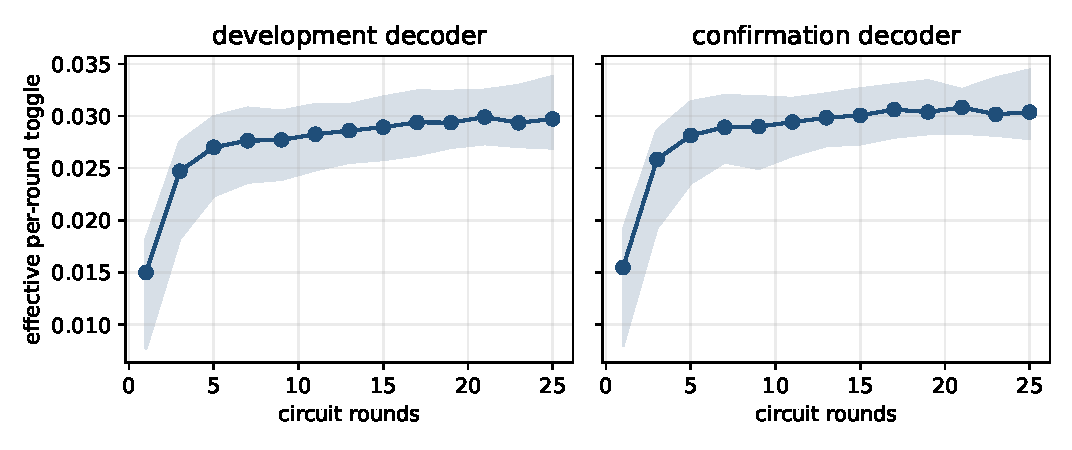
\includegraphics[width=\linewidth]{code/results/persistence/figures/effective_toggle_trajectories.pdf}
\caption{Mean effective toggle versus circuit depth for the development and
confirmation decoder endpoints. Shading spans the ten hardware strata. The
rapid rise through early rounds and continued later drift reject a single
depth-invariant toggle as a descriptive model of these records.}
\label{fig:trajectory}
\end{figure}

The effective toggle increases from approximately 0.015 at one round to about
0.030 at twenty-five rounds for both endpoints. The agreement of this pattern
across decoders supports a hardware-depth diagnostic rather than an artifact of
one decoder column. The stationary curve remains a relevant physics-based
baseline, but its misspecification is visible before forecast scores are
examined.

\subsection{Rolling prediction}

Figure~\ref{fig:rolling} presents every development fold and the unchanged
confirmation endpoint before the numerical summary in Table~\ref{tab:rolling}.

\begin{figure}[H]
\centering
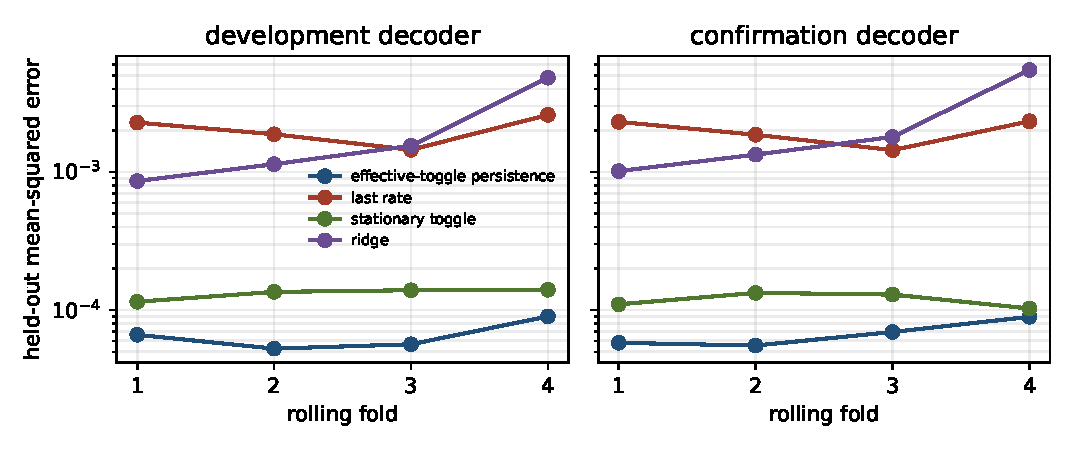
\includegraphics[width=\linewidth]{code/results/persistence/figures/rolling_error.pdf}
\caption{Held-out mean-squared error for all methods and all rolling folds.
The vertical scale is logarithmic. Effective-toggle persistence is best on
each development fold and on the unchanged confirmation endpoint.}
\label{fig:rolling}
\end{figure}

\begin{table}[H]
\centering
\caption{Rolling errors against the strongest comparator in each fold. MSE is
computed only on future depths; reduction is relative to the comparator MSE.}
\label{tab:rolling}
\scriptsize
\resizebox{\textwidth}{!}{%
\begin{tabular}{llrrrrr}
\toprule
endpoint & fold & test rounds & persistence MSE & strongest comparator & comparator MSE & reduction\\
\midrule
\PersistenceRows
\bottomrule
\end{tabular}}
\end{table}

The stationary toggle fit is the strongest comparator in every fold.
Development reductions range from 35.8 to 61.2 percent; confirmation reductions
range from 13.0 to 58.4 percent. Pairwise squared error favors persistence on
75--100 percent of development records and 62.5--95 percent of confirmation
records. The smaller final-fold confirmation margin is retained in
Table~\ref{tab:rolling}; it is not removed by redefining the horizon.

\begin{figure}[H]
\centering
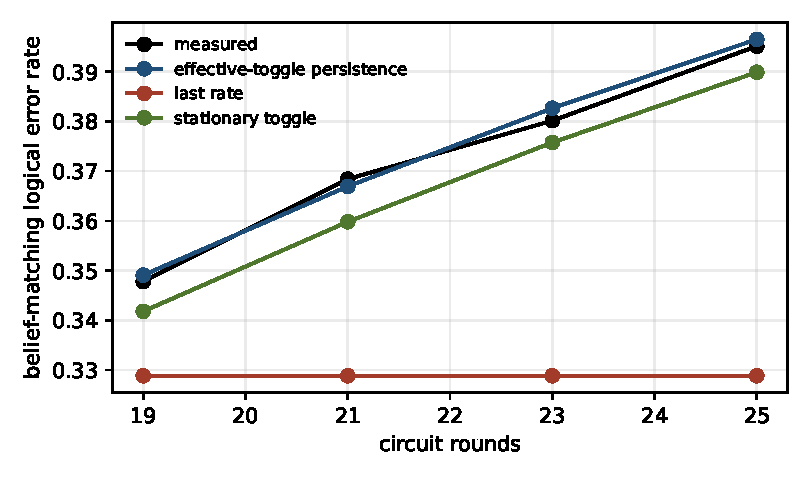
\includegraphics[width=0.78\linewidth]{code/results/persistence/figures/confirmation_forecast.pdf}
\caption{Final-fold belief-matching confirmation, averaged within round.
Carrying the raw last rate forward cannot represent continued accumulation.
The stationary fit remains systematically low. Effective-toggle persistence
tracks the measured curve at rounds 19--25.}
\label{fig:confirmation}
\end{figure}

Figure~\ref{fig:confirmation} explains the ranking rather than merely
displaying it. The last-rate baseline is flat by construction. The stationary
fit saturates too slowly because its single toggle compromises across earlier
depths. Persistence uses the latest effective state and preserves the parity
shape.

\subsection{Computational scaling}

Figure~\ref{fig:runtime} reports matched fit-and-predict timings on authentic
hardware strata; it is an implementation measurement rather than an asymptotic
claim.

\begin{figure}[H]
\centering
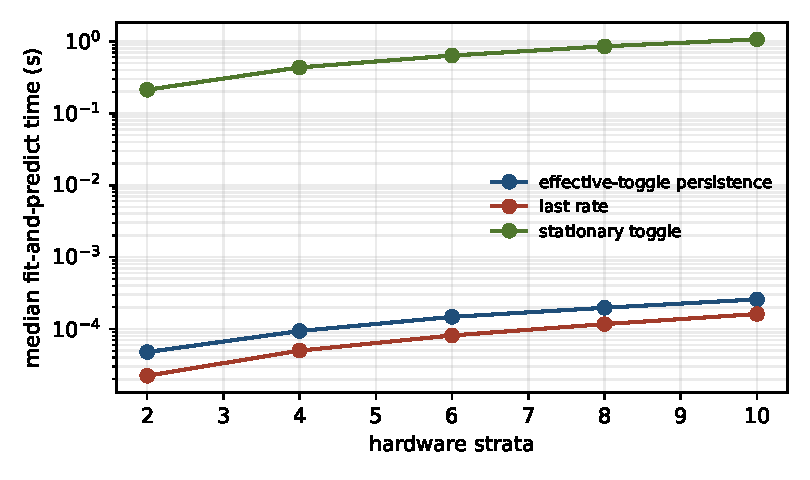
\includegraphics[width=0.78\linewidth]{code/results/persistence/figures/runtime_scaling.pdf}
\caption{Median fit-and-predict time versus the number of authentic hardware
strata. Persistence and last-rate timings use 101 repetitions; the
20,001-point stationary grid uses five. The plot reports this implementation,
not an intrinsic limit on optimized one-parameter fitting.}
\label{fig:runtime}
\end{figure}

At ten strata, persistence takes $2.58\times10^{-4}$ seconds in the recorded
run, the last-rate baseline takes $1.62\times10^{-4}$ seconds, and the streamed
grid fit takes 1.07 seconds. Proposition~\ref{prop:complexity} explains the
separation in this implementation. A specialized continuous optimizer could
substantially reduce the stationary baseline time; the scientific advantage of
persistence is its rolling accuracy and absence of a stationarity fit.

\section{Reproducibility and limitations}

The release contains the authenticated CSV file, parity transformations,
rolling-split implementation, strong baselines, theorem tests, timing arrays,
and the code generating every table and figure. The portable semantic digest
begins \texttt{fb0ff775}; timing and platform strings are excluded from that
digest and remain in the registered JSON record.

The data comprise one public hardware campaign and two decoder endpoints on the
same circuits. Confirmation across a decoder is not confirmation across a
device, calibration date, or code family. The estimator forecasts aggregate
logical rates and does not decode individual syndromes. Equation
\eqref{eq:drift-bound} is conditional on effective-toggle drift and is not a
probabilistic confidence interval. Later hardware campaigns, additional code
distances, and genuinely forward-collected rounds are required before a
deployment claim.

\section{Conclusion}

The parity transform exposes the variable that the stationary model assumes
constant. On the authenticated surface-code record, that effective toggle
drifts with circuit depth. Persisting its latest value preserves the bounded
accumulation geometry while avoiding numerical fitting. The resulting method
has linear work, one scalar state per hardware stratum, an explicit drift
bound, and lower rolling error on both decoder endpoints in all registered
folds. The contribution is a transparent forecasting rule and diagnostic for
depth-varying hardware records, with conclusions limited to the stated data.

\begin{thebibliography}{9}

\bibitem{dennis2002topological}
E. Dennis, A. Kitaev, A. Landahl, and J. Preskill,
Topological quantum memory,
\emph{J. Math. Phys.} \textbf{43} (2002), 4452--4505.

\bibitem{fowler2012surface}
A. G. Fowler, M. Mariantoni, J. M. Martinis, and A. N. Cleland,
Surface codes: towards practical large-scale quantum computation,
\emph{Phys. Rev. A} \textbf{86} (2012), 032324.

\bibitem{google2023suppressing}
Google Quantum collaborators,
Suppressing quantum errors by scaling a surface code logical qubit,
\emph{Nature} \textbf{614} (2023), 676--681.

\end{thebibliography}

\end{document}
